%!TEX root = ./main.tex

%%**************************************************************
%%
%% DHBW Stuttgart Campus Horb - Template for Bachelor Thesis & Project Thesis
%%
%% Bevor using this template please have a look at the REAMDME.md file
%%
%% Original Template found here:
%% https://github.com/schnes4/dhbw-heidenheim-latex-template
%% Modified for DHBW Stuttgart Campus Horb:
%% https://github.com/Vectabyte/dhbw-horb-latex-template
%%
%%**************************************************************

%!TEX root = ../main.tex

% show warning for old LaTeX syntax
\RequirePackage[l2tabu, orthodox]{nag}

\documentclass[
    pagesize=pdftex,        % Use pdfTeX page size settings
    twoside=false,          % Single-sided layout (was 'oneside')
    fontsize=12pt,          % Font size
    parskip=half,           % Space (in lines) between paragraphs
    headheight=12pt,        % Header height
    headsepline,            % Line after header
    footheight=16pt,        % Footer height
    footsepline,            % Line before footer
    abstract=true,          % Abstract headline
    DIV=calc,               % Calculate print space
    BCOR=8mm,               % BCOR setting (Bindekorrektur)
    headinclude=false,      % Exclude header from print space
    footinclude=false,      % Exclude footer from print space
    listof=totoc,           % Show List of Figures/Tables in Contents
    toc=bibliography        % Show Bibliography in Contents
]{scrreprt}                 % Koma-Script report-class, long document: scrreprt, short document: scrbook

\usepackage{xstring}
\usepackage[utf8]{inputenc}
\usepackage[T1]{fontenc}

% iflang command definition
\newcommand{\iflang}[2]{%
  \IfStrEq{\documentLanguage}{#1}{#2}{}%
}

% ifDocType comand definition
\newcommand{\ifDocType}[3]{%
  \IfStrEq{\documentType}{#1}{#2}{#3}%
}

% ifMultipleAuthors definition
\newcommand{\ifMultipleAuthors}[2]{%
  \IfStrEq{\multipleAuthors}{true}{#1}{#2}%
}

% ifRestrictionNotice definition
\newcommand{\ifRestrictionNotice}[2]{%
  \IfStrEq{\restrictionNotice}{true}{#1}{#2}%
}

% ifSpecialDocument definition
\newcommand{\ifSpecialDocument}[2]{\IfStrEqCase{\documentType}{%
	{T4\_1000}{#2\ignorespaces}%
	{T4\_2000}{#2\ignorespaces}%
	{T4\_3000}{#2\ignorespaces}%
	{T4\_3100}{#2\ignorespaces}%
	{T4\_3300}{#2\ignorespaces}%
	}[#1\ignorespaces]%
}

% Include main settings
%!TEX root = ../main.tex

%% Citation Styles
% http://ctan.mirrorcatalogs.com/macros/latex/contrib/biblatex/doc/biblatex.pdf (3.3.1 Citation Styles)
% recommended:  z.B numeric-comp, alphabetic, 
% not recommended: authoryear, alphabetic-verb, 
\newcommand{\quoteStyle}{alphabetic-verb}

%% Fonts
%% palatino, goudysans, lmodern or libertine
\newcommand{\documentFont}{lmodern}

%% Margin
\newcommand{\margin}{2.5cm}

%% Space between chapter headline and top of page
\newcommand{\chapterMargin}{20pt}

%% Table settings
% Column spacing
\newcommand{\tableColumnMargin}{10pt}
%Line spacing
\newcommand{\tableRowMargin}{1.5}

%% Color settings
\newcommand{\defineColors}{%
	\definecolor{LinkColor}{HTML}{\linkColor}
	\definecolor{ListingBackground}{HTML}{F8F8F8}
}

%% Syntax Highlighting (Listings)
\newcommand{\listingsettings}{%
	\lstset{%
		aboveskip=20pt,
		backgroundcolor=\color{ListingBackground}, % source code background color
		basicstyle=\ttfamily\footnotesize, % the size of the fonts that are used for the code
		breakautoindent=true,	        % indenting after break line (true, false)
		breakatwhitespace=false,         % sets if automatic breaks should only happen at whitespace
		breaklines=true,		        % break lines if necessary (true, false), sets automatic line breaking
		captionpos=b,			% sets the caption-position to bottom
		commentstyle=\color[rgb]{0.133,0.545,0.133}, % comment style
		deletekeywords={...},            % if you want to delete keywords from the given language
		escapeinside={\%*}{*)},          % if you want to add LaTeX within your code
		extendedchars=true,		% show all Latin1 characters (true, false), lets you use non-ASCII characters; for 8-bits encodings only, does not work with UTF-8
		firstnumber=1,                % start line enumeration with line X
		fillcolor=\color{ListingBackground},
		frame=single,			        % adds a frame around the code
		frameround=ffff,
		keepspaces=true,                 % keeps spaces in text, useful for keeping indentation of code (possibly needs columns=flexible)
		keywordstyle=\color[rgb]{0.133,0.133,0.6}, % keyword style
		language=Java,			% default language
		morekeywords={*,...},            % if you want to add more keywords to the set
		numbers=left,			% where to put the line-numbers; possible values are (none, left, right)
		numbersep=5pt,			% 5pt between number and source code, how far the line-numbers are from the code
		numberstyle=\tiny,		% letter size of numbers, the style that is used for the line-numbers
		postbreak=\space,		% break line after space
		rulecolor=\color{darkgray},	% border color, if not set, the frame-color may be changed on line-breaks within not-black text (e.g. comments (green here))
		showspaces=false,		% show spaces everywhere adding particular underscores; it overrides 'showstringspaces' (true, false)		
		showstringspaces=false,	% underline spaces within strings only (true, false)
		showtabs=false,                  % show tabs within strings adding particular underscores
		stepnumber=1,			% the step between two line-numbers. If it's 1, each line will be numbered
		stringstyle=\color[rgb]{0.627,0.126,0.941}, % string literal style
		tabsize=2,				% sets default tabsize to 2 spaces
		xleftmargin=10pt,		        % margin left
		xrightmargin=5pt,		        % margin right
	}
}
 

% Include document settings
%!TEX root = ../main.tex

%% Document language (en, de)
\newcommand{\documentLanguage}{de}

%% Document type
% T4\_1000 Project Thesis (Semester 1 & 2)
% T4\_2000 Project Thesis (Semester 3 & 4)
% T4\_3000 Project Thesis (Semester 5 & 6)
% T4\_3100 Seminar Paper (Semester 5 & 6)
% T4\_3300 Bachelor Thesis
\newcommand{\documentType}{T4\_1000}
\newcommand{\restrictionNotice}{false}

\newcommand{\aiUsed}{true}

\newcommand{\multipleAuthors}{false}
\newcommand{\documentAuthor}{Max Mustermann}
\newcommand{\documentTitle}{Titel der Arbeit}
\newcommand{\documentPeriod}{8 Wochen}

\newcommand{\matriculationNumber}{12345678}

\newcommand{\locationUniversity}{Stuttgart Campus Horb}
\newcommand{\department}{Informatik}
\newcommand{\course}{HOR-TINF2024}

\newcommand{\degree}{Bachelor of Science}
% INF2014 - INF2016 (MI):       Bachelor of Science
% INF2014 - INF2016 (IA/IM) :   Bachelor of Engineering
% INF2017 (all):                Bachelor of Science
% TINF2024:                     Bachelor of Science

% A lecture that the document is written for
\newcommand{\lecture}{Software Engineering}
% Whether to show the lecture on cover
\newcommand{\showLecture}{false}

\newcommand{\releaseDate}{XX. September 20XX}
\newcommand{\releaseLocation}{Standort Abgabe}

\newcommand{\companyName}{Firma}
\newcommand{\companyLocation}{Standort}

\newcommand{\tutor}{Betreuer}
\newcommand{\evaluator}{Prof. Dr.-Ing. Someone Name}

\newcommand{\linkColor}{00007A}


% Load language specific Strings
\input{lang/\documentLanguage}

% Load language specific babel package
\iflang{de}{\usepackage[english, ngerman]{babel}}
\iflang{en}{\usepackage[ngerman, english]{babel}} 

% Add comment feature
\newcommand{\comment}[1]{\par {\bfseries \color{blue} #1 \par}}


%%%%%%% Package Includes %%%%%%%

\usepackage[margin=\margin,foot=1cm]{geometry}
\usepackage[activate]{microtype}                                         
\usepackage[onehalfspacing]{setspace}
\usepackage{makeidx}
\usepackage[autostyle=true,german=quotes]{csquotes}
\usepackage{longtable}
\usepackage{enumitem}	                                                 
\usepackage{graphicx}
\usepackage{pdfpages}                                                         
\usepackage{xcolor} 	                                                    
\usepackage{float}
\usepackage{array}
\usepackage{calc}		                         
\usepackage[right]{eurosym}
\usepackage{wrapfig}
\usepackage{pgffor}                                                             
\usepackage[perpage, hang, multiple, stable]{footmisc}  
\usepackage[printonlyused]{acronym}                                 
\usepackage{listings}
\usepackage[obeyFinal,backgroundcolor=yellow,linecolor=black]{todonotes}
\usepackage{rotating}
\usepackage{lscape}
\usepackage{amsmath}
\usepackage{amssymb}
\usepackage{\documentFont}
\usepackage[hyphens]{url}

% Bibliographie settings
\iflang{de}{%
\usepackage[
	backend=biber,		% recommended. Alternative: bibtex
	bibwarn=true,
	bibencoding=utf8,	         % If .bib file is encoded with utf8, otherwise ascii
	sortlocale=de_DE,
	url=true,
	style=\quoteStyle,
]{biblatex}
}
\iflang{en}{%
\usepackage[
	backend=biber,		% recommended. Alternative: bibtex
	bibwarn=true,
	bibencoding=utf8,        % If .bib file is encoded with utf8, otherwise ascii
	sortlocale=en_US,
	url=true,
	style=\quoteStyle,
]{biblatex}
}

\addbibresource{bibliographie.bib}

% hyperreferences and links
\usepackage[%
	pdftitle={\documentTitle},
	pdfauthor={\documentAuthor},
	pdfsubject={\documentType},
	pdfcreator={pdflatex, LaTeX with KOMA-Script},
	pdfpagemode=UseOutlines,       % Show Contents while opening
	pdfdisplaydoctitle=true, 		% Show document title instead of file name
	pdflang={\documentLanguage}, % Document language
]{hyperref}
\restylefloat{figure}
\usepackage{caption}
\usepackage[all]{hypcap}
\usepackage{bookmark}
\usepackage[nonumberlist,toc,acronym]{glossaries}
\usepackage[nonumberlist,toc]{glossaries}
\usepackage{scrhack}

% Generate glossary
\makeglossaries{}

% Load colors
\defineColors{}

% Set Titel, Autor and Date
\title{\documentTitle}
\author{\documentAuthor}
\date{\datum}


% PDF link settings
\hypersetup{%
	colorlinks=true, 		
	linkcolor=LinkColor, 	
	citecolor=LinkColor,
	filecolor=LinkColor,
	menucolor=LinkColor,
	urlcolor=LinkColor,
	linktocpage=true, 
	bookmarksnumbered=true 
}

% Captions fontsize
\addtokomafont{caption}{\small}

% die letzte Zeile eines Absatzes steht auf einer neuen Seite und Seitenumbruch nach der ersten Zeile eines neuen Absatzes verhindern
% http://projekte.dante.de/DanteFAQ/Silbentrennung
\clubpenalty = 10000 % schließt Seitenumbruch nach der ersten Zeile eines neuen Absatzes aus
\widowpenalty = 10000 % schließt die letzte Zeile eines Absatzes steht auf einer neuen Seite aus
\displaywidowpenalty=10000

% Graphicspath
\graphicspath{{images/}}

% frequently used programing languages
% for More see Page 12 of https://ftp.agdsn.de/pub/mirrors/latex/dante/macros/latex/contrib/listings/listings.pdf
\lstloadlanguages{
  PHP,
  Python,
  Java,
  C,
  [ISO]C++,   % Optional: [ISO] kann entfernt werden
  [Sharp]C,        % Für C#
  bash,
  HTML,
  SQL
}
\iffalse
Default, if set, listed in brackets at the end
to set a different dialect: [dialect]language e.g. [Sharp]C

List of Programming Languages

ABAP (R/2 4.3, R/2 5.0, R/3 3.1, R/3 4.6C, R/3 6.10)(Default: R/3 6.10)
ACM 
ACMscript
ACSL 
Ada (2005, 83, 95)(Default: 2005)
Algol (60, 68)(Default: 68)
Ant
Assembler (Motorola68k, x86masm) 
Awk (gnu, POSIX)(Default: gnu)
bash 
Basic (Visual)
C (ANSI, Handel, Objective, Sharp)(Default: ANSI)
C++ (11, ANSI, GNU, ISO, Visual)(Default: ISO)
Caml (light, Objective)(Default: light)
CIL 
Clean
Cobol (1974, 1985, ibm)(Default: 1985)
Comal 80
command.com (WinXP)(Default: WinXP) 
Comsol
csh 
Delphi
Eiffel 
Elan
elisp 
erlang
Euphoria 
Fortran (03, 08, 18, 77, 90, 95)(Default: 95)
GAP 
GCL
Gnuplot 
Go
hansl 
Haskell
HTML 
IDL (empty, CORBA)
Inform 
Java (empty, AspectJ)
JVMIS 
ksh
Lingo 
Lisp (empty, Auto)
LLVM 
Logo
Lua (5.0, 5.1, 5.2, 5.3)(Default: 5.3) 
make (empty, gnu)
Mathematica (1.0, 11.0, 3.0, 5.2)(Default: 11.0)
Matlab (empty, 5.1)
Mercury 
MetaPost
Miranda 
Mizar
ML 
Modula-2
MuPAD 
NASTRAN
Oberon-2 
OCL (decorative, OMG)(Default: OMG)
Octave 
OORexx
Oz 
Pascal (Borland6, Standard, XSC)(Default: Standard)
Perl 
PHP
PL/I 
Plasm
PostScript 
POV
Prolog 
Promela
PSTricks 
Python (2, 3)(Default: 2)
R 
Reduce
Rexx (empty, VM/XA) 
RSL
Ruby 
S (empty, PLUS)
SAS 
Scala (empty, 3.0)
Scilab 
sh
SHELXL 
Simula (67, CII, DEC, IBM)(Default: 67)
SPARQL 
SQL
Swift 
tcl (empty, tk)
TeX (AlLaTeX, common, LaTeX, plain, primitive)(Default: plain)
VBScript 
Verilog
VHDL (empty, AMS) 
VRML (97)(Default: 97)
XML 
XSLT
\fi

\listingsettings{}
% Rename Listings
\renewcommand\lstlistingname{\listingPhrase} % sets the Phrase below a Listing e.g. Listing 1
\renewcommand\lstlistlistingname{\listListingPhrase} % sets the Title of the Listlistings Page e.G. List of Listings
\def\lstlistingautorefname{\autrefListingPhrase} % sets the Phrase inserted when using \autoref to reference a Listing e.g. this \autoref{labelname} -> this Listing 1

% Spaces in tables
\setlength{\tabcolsep}{\tableColumnMargin}
\renewcommand{\arraystretch}{\tableRowMargin}




%!TEX root = ../main.tex

%
% To create glossary run the following command: 
% makeglossaries main.acn && makeglossaries main.glo
%

%
% Glossareintraege --> referenz, name, beschreibung
% Aufruf mit \gls{...}
%
\newglossaryentry{Glossareintrag}{
    name={Glossareintrag},
    plural={Glossareinträge},
    description={Ein Glossar beschreibt verschiedenste Dinge in kurzen Worten}
    }


\begin{document}

	\pagenumbering{arabic}

	% Cover
	\begin{spacing}{1}
		%!TEX root = ../main.tex

\begin{titlepage}
	\begin{longtable}{p{8cm} p{8cm}}
		\raggedright {\raisebox{\ht\strutbox-\totalheight}{
\includegraphics[height=2.5cm]{images/cover/logo-dhbw.pdf}}} &
		% no company logo for semester paper and special documents
		\ifDocType{T4\_3100}{}{%
			\ifSpecialDocument{}{%
				\raggedleft {\raisebox{\ht\strutbox-\totalheight}{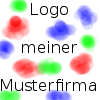
\includegraphics[height=2.5cm]{images/cover/logo-company.png}}}
			}%
		}%
	\end{longtable}
	\enlargethispage{20mm}
	\begin{center}
		\doublespacing{
		\vspace*{12mm}	{\LARGE\textbf \documentTitle }}\\
		\vspace*{12mm}	{\large\textbf {\documentTypePhrase}}\\
		
		% degree only for bachelor thesis
		\ifDocType{T4\_3300}{
			\vspace*{12mm}	\degreePhrase\\
			\vspace*{3mm}		{\textbf \degree}\\
		}

		\IfStrEq{\showLecture}{true}{
			\vspace*{12mm}	\lecturePhrase\\
			\vspace*{0mm}		{\textbf \lecture}\\
		}

		\vspace*{12mm}	\departmentPhrase{} \department\\
    \vspace*{0mm}		\locationUniversityPhrase{} \locationUniversity\\
		\vspace*{12mm}	\documentAuthorPhrase\\
		\vspace*{3mm}		{\large\textbf \documentAuthor}\\
		\vspace*{12mm}	\releaseDate\\
	\end{center}
	\vfill
	\begin{spacing}{1.2}
	\begin{tabbing}
		mmmmmmmmmmmmmmmmmmmmmmmmmm             \= \kill
		\textbf{\documentPeriodPhrase}       \>  \documentPeriod\\
		\textbf{\matriculationNumberPhrase, \coursePhrase}  \>  \matriculationNumber, \course\\

		% no company for the semester paper and special documents
		\ifDocType{T4\_3100}{}{%
			\ifSpecialDocument{}{%
				\textbf{\companyPhrase}                  \>  \companyName, \companyLocation\\
			}%
		}%
		\textbf{\tutorPhrase}               \>  \tutor\\

		% evaluator only for bachelor thesis
		\ifDocType{T4\_3300}{%
			\textbf{\evaluatorPhrase}              \>  \evaluator
		}{}
	\end{tabbing}
	\end{spacing}
\end{titlepage}

	\end{spacing}
	\newpage

	% Restriction notices
	\ifRestrictionNotice{%
		\ifDocType{T4\_3100}{%
			% no restricition notices for semester paper
		}{%
			%!TEX root = ../main.tex

\thispagestyle{empty}

\section*{\restrictionNoticesPhrase}

\vspace*{2em}

\iflang{de}{%
  Die vorliegende {\documentTypePhrase} mit dem Titel \textit{\documentTitle} beinhaltet interne und vertrauliche Informationen der Firma {\companyName}. 

  \textbf {Die Veröffentlichung sowie jede sonstige Weitergabe des Inhalts der Arbeit und eventuelle beiliegender Zeichnungen und Daten,
  im Gesamten oder in Teilen ist, mit Ausnahme der beteiligten Mitglieder des Prüfungsausschusses, grundsätzlich untersagt.
  Es dürfen keinerlei Kopien oder Abschriften - auch nicht in elektronischer Form - angefertigt werden.}

  Ausnahmen bedrüfen der schriftlichen Genehmigung der Firma {\companyName}.
}

\iflang{en}{%
  The present {\documentTypePhrase} titled \textit{\documentTitle} contains internal and confidential information of {\companyName}.

  \textbf {The publication or any other disclosure of the contents of this document and any accompanying drawings and data,
  in whole or in part, is strictly prohibited, with the exception of the members of the examination committee involved.
  No copies or transcripts may be made, including in electronic form.}

  Exceptions require the written approval of the company {\companyName}.
}

\vspace{3em}

\releaseLocation, \releaseDate
\vspace{4em}

\rule{6cm}{0.4pt}\\
\documentAuthor

			\newpage
		}%
	}{}

	% Declaration
	%!TEX root = ../main.tex

\thispagestyle{empty}

\section*{\declarationPhrase}

\vspace*{2em}

\iflang{de}{%
  \ifMultipleAuthors{Wir versichern}{Ich versichere} hiermit, dass \ifMultipleAuthors{wir unsere}{ich meine} 
  {\documentTypePhrase} mit dem Thema: \textit{\documentTitle} 
  selbstständig verfasst und keine anderen als die angegebenen Quellen und Hilfsmittel benutzt \ifMultipleAuthors{haben}{habe}. 
  \ifMultipleAuthors{Wir versichern}{Ich versichere} zudem, dass die eingereichte elektronische Fassung mit der gedruckten Fassung 
  übereinstimmt. \ifAIUsed{\ifMultipleAuthors{Wir haben}{Ich habe} bei der Erstellung der Arbeit KI-Werkzeuge eingesetzt. Dies \ifMultipleAuthors{haben wir}{habe ich} in der \textbf{\aiacknowledgementPhrase}  zusammenfassend dokumentiert.}{}
}


\iflang{en}{%
  Hereby \ifMultipleAuthors{we}{I} solemnly declare:
  \begin{enumerate}
  \item that this {\documentTypePhrase}, titled \textit{\documentTitle} is entirely the product of \ifMultipleAuthors{our}{my} 
            own scholarly work, unless otherwise indicated in the text or references, or acknowledged below;
  \item \ifMultipleAuthors{we}{I} have indicated the thoughts adopted directly or indirectly from other sources at the appropriate 
            places within the document;
  \item this {\documentTypePhrase} has not been submitted either in whole or part, for a degree at this or 
            any other university or institution;
  \item \ifMultipleAuthors{we}{I} have not published this {\documentTypePhrase} in the past;
  \item the printed version is equivalent to the submitted electronic one.
  \end{enumerate}
  \ifMultipleAuthors{We are}{I am} aware that a dishonest declaration will entail legal consequences.
  \ifAIUsed{\ifMultipleAuthors{We have}{I have} used AI tools in the creation of this work. This has been documented in the \textbf{\aiacknowledgementPhrase} section.}{}
}

\vspace{3em}

\releaseLocation, \releaseDate
\vspace{4em}

\rule{6cm}{0.4pt}\\
\documentAuthor

	\newpage

	% Abstract
	%!TEX root = ../main.tex

\pagestyle{empty}

% override abstract headline
\renewcommand{\abstractname}{Abstract}

\begin{abstract}
Insert your Abstract here!
\end{abstract}
	\newpage

    % only page number in footer
	\pagestyle{plain}
	
	% space bevore chapter headline
	\RedeclareSectionCommand[beforeskip=\chapterMargin]{chapter}

	% Contents
	\begin{spacing}{1.1}
		\begingroup
		
		    % set subchapter depth
			\setcounter{tocdepth}{1} % set subchapter depth (0=chapter, 1=section, 2=subsection, 3=subsubsection), Setting to 2 to show only up to subsection level (e.g., 6.1.1 but not 6.1.1.2)
			\pagestyle{empty}	
			\tableofcontents
			\addtocontents{toc}{\protect\thispagestyle{empty}}
			\clearpage
		\endgroup
	\end{spacing}
	\newpage

	%\pagenumbering{arabic}
	
	\pagestyle{headings}

	% Change numbering from 1.1, 1.2, 2.1 to 1, 2, 3

	% Change figure numbering to be continuous throughout the document e.g. Figure 1, Figure 2, ... instead of Figure 1.1, Figure 1.2, Figure 2.1, ... (with chapter number as prefix)
	\makeatletter
	\@removefromreset{figure}{chapter}
	\makeatother
	\renewcommand{\thefigure}{\arabic{figure}}

	% Change lstlisting numbering to be continuous throughout the document e.g. Listing 1, Listing 2, ... instead of Listing 1.1, Listing 1.2, Listing 2.1, ... (with chapter number as prefix)
	\makeatletter
	\@removefromreset{lstlisting}{chapter}
	\makeatother
	\renewcommand{\thelstlisting}{\arabic{lstlisting}}

	% Change table numbering to be continuous throughout the document e.g. Table 1, Table 2, ... instead of Table 1.1, Table 1.2, Table 2.1, ... (with chapter number as prefix)
	\makeatletter
	\@removefromreset{table}{chapter}
	\makeatother
	\renewcommand{\thetable}{\arabic{table}}
	\setcounter{table}{0}

	%Content
	\foreach \i in {01,02,03,04,05,06,07,08,09,...,99} {%
		\edef\FileName{content/chapter/\i .tex}%
			\IfFileExists{\FileName}{%
				\input{\FileName}
			}
			{%
%				No chapter available
			}
	}

	\clearpage
	
	%\pagenumbering{Roman}

	% Appendix
	\clearpage
	\appendix
	% !TeX root = ../main.tex

\addchap{\appendixPhrase}




	% Glossar
	\cleardoublepage
	\newpage % needed to make the next line work correctly
	\pagenumbering{Roman} % Set Numbering to Roman and start counting from 1 (I) again
	\printglossary[style=altlist,title=\glossaryPhrase]
	%!TEX root = ../main.tex

%
% To create glossary run the following command: 
% makeglossaries main.acn && makeglossaries main.glo
%

%
% Glossareintraege --> referenz, name, beschreibung
% Aufruf mit \gls{...}
%
\newglossaryentry{Glossareintrag}{
    name={Glossareintrag},
    plural={Glossareinträge},
    description={Ein Glossar beschreibt verschiedenste Dinge in kurzen Worten}
    }


	% Bibilography
	\cleardoublepage
	\begingroup
	\sloppy % used to adjust some Bibliography visuals e.g. not writing beyond the right hand side to have a clean break
	\printbibliography
	\endgroup

	% List of Figures
	\cleardoublepage
	\listoffigures

	%List of Tables
	\cleardoublepage
	\listoftables

	% List of Listings
	\cleardoublepage
	\lstlistoflistings
	\cleardoublepage

	% Acronyms
	\cleardoublepage
    %!TEX root = ../main.tex

\addchap{\acronymsPhrase}

\begin{acronym}[XXXXX] % Set XXXXX to the length of your longest Acronym by adding or removing X's, in this case longest Acronym is 5
% \setlength{\itemsep}{-\parsep} % use if you dont want any spaces between your definitions       

\acro{AGPL}[AGPL]{Affero GNU General Public License} % Reference to call back in your document with \ac{XXXX}, Acronym, Long form of said acronym

\end{acronym}

	
\end{document}
